%!TEX root = Slic3r-Manual.tex
\subsection{Working with Models}
\label{sub:working_with_models}
\index{models}

Yet another step lies between now and the first print - a model has to found and then sliced.

\subsubsection{Model Formats} % (fold)
\label{sub:model_formats}
\index{STL}
\index{AMF}
\index{OBJ}

Slic3r accepts the following file types.

\begin{itemize}
	\item STereoLithography (STL) files can come from a wide variety of sources and are now a de facto standard in 3D printing.  The files simply describe the surface geometry of a 3D object without any additional information (such as color or material), and it is this simplicity that has probably made the format ubiquitous.
	\item Wavefront OBJ files are an open format originally used in an animation application from Wavefront Technologies, but has since been adopted by the wider 3D modelling community.  It is similar to the STL format.
	\item Additive Manufacturing File Format (AMF) was developed in response to the limited nature of the STL format.  In addition to describing the geometry of the 3D model it can also describe colors and materials, as well as more complex attributes, such as gradient mixes and multiple object arrangements (constellations).  Whilst the format is deemed a standard it has yet to be widely adopted in the 3D maker community.
\end{itemize}
% subsubsection model_formats (end)

\subsubsection{Finding Models} % (fold)
\label{sub:finding_models}
\index{models!finding}

The 3D model files may come from an online repository, such as Thingiverse\footnote{http://www.thingiverse.com} or GrabCAD\footnote{http://grabcad.com}, or be created from a CAD program, such as FreeCAD\footnote{http://sourceforge.net/projects/free-cad}, Sketchup\footnote{http://www.sketchup.com}, or OpenSCAD\footnote{http://www.openscad.org}, or an online CAD tool such as Shapesmith\footnote{http://shapesmith.net}.

You may wish to view the files before slicing and there are many free applications available, one of which is Meshlab\footnote{http://www.meshlab.org} - a comprehensive tool for viewing and working with 3D files.

\begin{figure}[H]
\centering
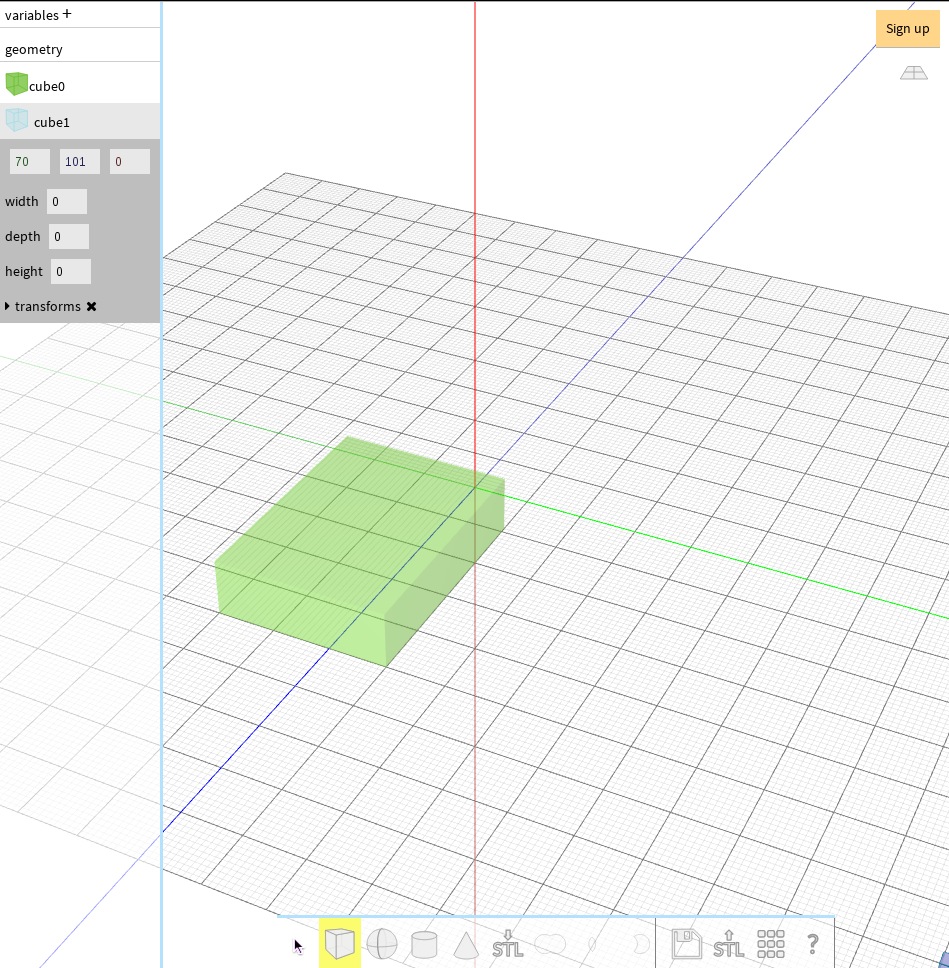
\includegraphics[keepaspectratio=true,width=0.75\textwidth]{working_with_models/shapesmith.png}
\caption{Shapesmith online CAD tool.}
\label{fig:shapesmith}
\end{figure}

% subsubsection working_with_models (end)


\subsubsection{Working with Plater} % (fold)
\label{sub:working_with_plater}
\index{Plater}
Slic3r has a tool, called Plater, which allows one or more models to be loaded and arranged before being sliced.

\begin{figure}[H]
\centering
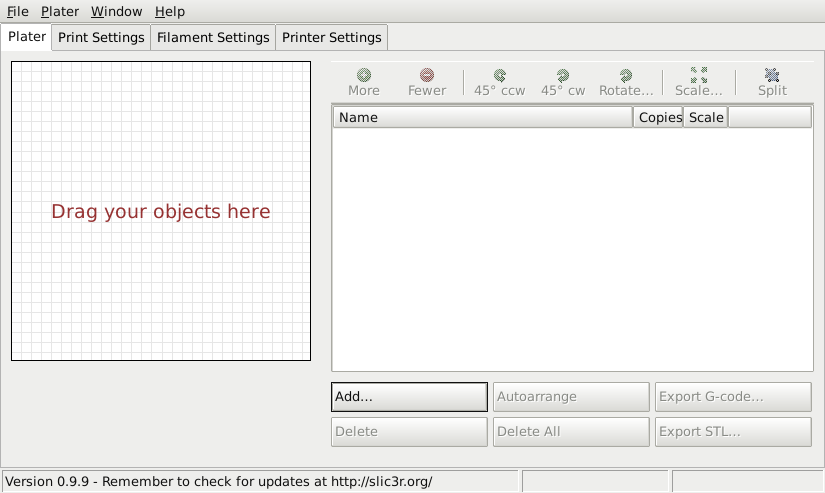
\includegraphics[keepaspectratio=true,width=1\textwidth]{working_with_models/plater.png}
\caption{Plater}
\label{fig:plater}
\end{figure}

Once you have acquired a model, drag it onto the Plater window (or use the Add button below the file list) to load it into Slic3r.  In the figure below, the traditional RepRap Minimug\footnote{http://www.thingiverse.com/thing:18357} is loaded, and is viewed from above. The ring around the model is a skirt - a single perimeter, several millimeters away from the model, which is extruded first.  This is useful in making sure the plastic is flowing smoothly from the nozzle when the model is starting to be printed.

\begin{figure}[H]
\centering
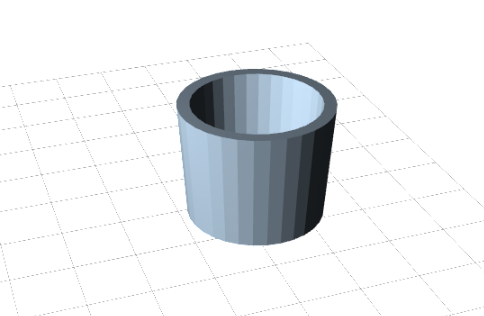
\includegraphics[keepaspectratio=true,width=0.75\textwidth]{working_with_models/minimug_model.png}
\caption{Minimug model.}
\label{fig:minimug_model}
\end{figure}

\begin{figure}[H]
\centering
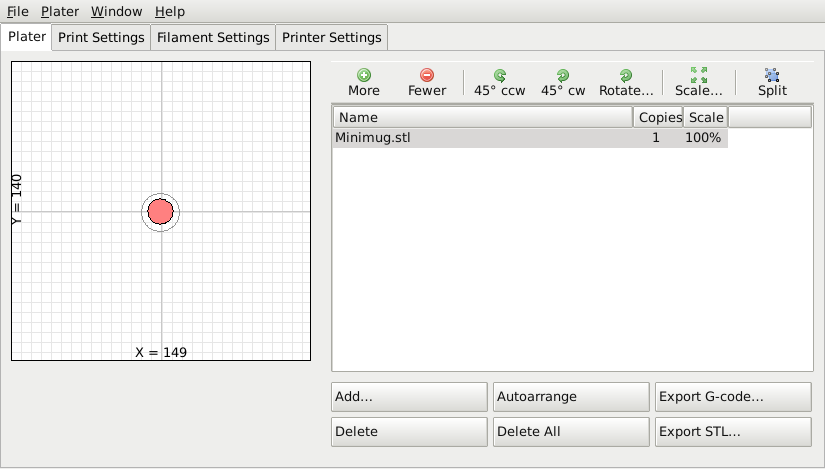
\includegraphics[keepaspectratio=true,width=1\textwidth]{working_with_models/plater_model_loaded.png}
\caption{STL file loaded.}
\label{fig:plater_model_loaded}
\end{figure}

The model can be repositioned by dragging the representation of it on the left of the screen around the bed.  Note that the dimensions of the bed should match your printer, as given during the initial configuration above.

On the right-hand side is the list of currently loaded files.  The buttons along the top of the file list allow you to arrange the models.
\begin{itemize}
	\item \textbf{More/Less}  - Adjust how many copies should be printed.
	\item \textbf{45°/Rotate}  - Rotate the selected model around the Z axis, either in 45° increments clockwise or counter-clockwise, or by a given amount.
	\item \textbf{Scale}  - Increase or decrease the size of the printed model.
	\item \textbf{Split}  - Divides a model which consists of more than one part into it's constituent parts, allowing each one to be arranged individually.
\end{itemize}

The buttons along the bottom of the file list allow you to add, remove, auto-arrange, or export the models.
\begin{itemize}
	\item \textbf{Add}  - Opens a file dialog to add a model to the plater, as an alternative to dropping a file directly.
	\item \textbf{Delete/Delete All}  - Remove one or all models from the plater.
	\item \textbf{Autoarrange}  - Attempt to arrange the models to give the optimal layout.
	\item \textbf{Export G-code}  - Starts slicing the model and produces a G-Code file.
	\item \textbf{Export STL}  - Save the current set of models as a single STL file.
\end{itemize}


% subsubsection working_with_plater (end)

\subsubsection{Cleaning STLs} % (fold)
\label{sub:cleaning_stls}
\index{STL!cleaning}
If the 3D mesh described in the model contains holes, or edges are misaligned (known as being non-manifold), then Slic3r may have problems working on it.  Slic3r will attempt to fix any problems it can, but some problems are out of its reach.  If the application complains that a model cannot be sliced correctly then there are several options available: see the chapter about Repairing Models.

% subsubsection cleaning_stls (end)
